% mnras_template.tex 
%
% LaTeX template for creating an MNRAS paper
%
% v3.0 released 14 May 2015
% (version numbers match those of mnras.cls)
%
% Copyright (C) Royal Astronomical Society 2015
% Authors:
% Keith T. Smith (Royal Astronomical Society)

% Change log
%
% v3.2 July 2023
%	Updated guidance on use of amssymb package
% v3.0 May 2015
%    Renamed to match the new package name
%    Version number matches mnras.cls
%    A few minor tweaks to wording
% v1.0 September 2013
%    Beta testing only - never publicly released
%    First version: a simple (ish) template for creating an MNRAS paper

%%%%%%%%%%%%%%%%%%%%%%%%%%%%%%%%%%%%%%%%%%%%%%%%%%
% Basic setup. Most papers should leave these options alone.
\documentclass[fleqn,usenatbib]{mnras}

% MNRAS is set in Times font. If you don't have this installed (most LaTeX
% installations will be fine) or prefer the old Computer Modern fonts, comment
% out the following line
\usepackage{newtxtext,newtxmath}
% Depending on your LaTeX fonts installation, you might get better results with one of these:
%\usepackage{mathptmx}
%\usepackage{txfonts}

% Use vector fonts, so it zooms properly in on-screen viewing software
% Don't change these lines unless you know what you are doing
\usepackage[T1]{fontenc}

% Allow "Thomas van Noord" and "Simon de Laguarde" and alike to be sorted by "N" and "L" etc. in the bibliography.
% Write the name in the bibliography as "\VAN{Noord}{Van}{van} Noord, Thomas"
\DeclareRobustCommand{\VAN}[3]{#2}
\let\VANthebibliography\thebibliography
\def\thebibliography{\DeclareRobustCommand{\VAN}[3]{##3}\VANthebibliography}


%%%%% AUTHORS - PLACE YOUR OWN PACKAGES HERE %%%%%

% Only include extra packages if you really need them. Avoid using amssymb if newtxmath is enabled, as these packages can cause conflicts. newtxmatch covers the same math symbols while producing a consistent Times New Roman font. Common packages are:
\usepackage{graphicx}	% Including figure files
\usepackage{amsmath}	% Advanced maths commands
\usepackage[dvipsnames,svgnames,x11names]{xcolor}
\usepackage{tikz}
\usetikzlibrary{graphs,shapes.geometric,patterns,decorations.pathreplacing}

%%%%%%%%%%%%%%%%%%%%%%%%%%%%%%%%%%%%%%%%%%%%%%%%%%

%%%%% AUTHORS - PLACE YOUR OWN COMMANDS HERE %%%%%

% Please keep new commands to a minimum, and use \newcommand not \def to avoid
% overwriting existing commands. Example:
%\newcommand{\pcm}{\,cm$^{-2}$}	% per cm-squared

% Distributions
\newcommand{\normaldist}{\mathcal{N}}
\newcommand{\uniformdist}{\mathcal{U}}
\newcommand{\gammadist}{\Gamma}
\newcommand{\tdist}{\mathcal{T}}

\renewcommand*{\vec}[1]{\boldsymbol{#1}}
\newcommand*{\mat}[1]{\boldsymbol{\mathsf{#1}}}
\newcommand*{\transpose}{\mathsf{T}}

% Model Parameters
\newcommand{\obs}{{y}}
\newcommand{\inputs}{{x}}
\newcommand{\outputs}{{u}}
\newcommand{\pred}{{\tilde{\outputs}}}
\newcommand{\error}{{\delta}}

\newcommand{\dydz}{\ensuremath{m_Y}}
\newcommand{\yp}{\ensuremath{c_Y}}

\newcommand{\eep}{\ensuremath{s}}
\newcommand{\feh}{\ensuremath{\mathrm{[Fe/H]}}}
\newcommand{\mlt}[1][]{{\ensuremath{\alpha_{\mathrm{mlt} \ifx#1\empty \else , #1 \fi}}}}
\newcommand{\teff}[1][]{{\ensuremath{T_{\mathrm{eff} \ifx#1\empty \else , #1 \fi}}}}

% Units
\newcommand{\solarmass}{\ensuremath{\mathrm{M}_\odot}}

%%%%%%%%%%%%%%%%%%%%%%%%%%%%%%%%%%%%%%%%%%%%%%%%%%

%%%%%%%%%%%%%%%%%%% TITLE PAGE %%%%%%%%%%%%%%%%%%%

% Title of the paper, and the short title which is used in the headers.
% Keep the title short and informative.
\title[Scalable stellar inference]{[TBC] Scalable stellar inference: hierarchical Bayesian framework with a neural network surrogate model for stellar evolution}

% The list of authors, and the short list which is used in the headers.
% If you need two or more lines of authors, add an extra line using \newauthor
\author[A. J. Lyttle et al.]{
Alexander J. Lyttle,$^{1}$\thanks{E-mail: a.j.lyttle@bham.ac.uk (AJL)}
Guy R. Davies,$^{1}$
Owen J. Scutt,$^{1}$
Yaguang Li,$^{2}$
Amalie Stokholm,$^{1}$
and Tanda Li$^{3}$
\\
% List of institutions
$^{1}$School of Physics and Astronomy, University of Birmingham, Birmingham B15 2TT, UK\\
$^{2}$Hawaii\\
$^{3}$Beijing
}

% These dates will be filled out by the publisher
\date{Accepted XXX. Received YYY; in original form ZZZ}

% Enter the current year, for the copyright statements etc.
\pubyear{2024}

% Don't change these lines
\begin{document}
\label{firstpage}
\pagerange{\pageref{firstpage}--\pageref{lastpage}}
\maketitle

% Abstract of the paper
\begin{abstract}

\end{abstract}

% Select between one and six entries from the list of approved keywords.
% Don't make up new ones.
\begin{keywords}
methods: statistical -- stars: fundamental parameters -- stars: low-mass
\end{keywords}

%%%%%%%%%%%%%%%%%%%%%%%%%%%%%%%%%%%%%%%%%%%%%%%%%%

%%%%%%%%%%%%%%%%% BODY OF PAPER %%%%%%%%%%%%%%%%%%

\section{Introduction}

Recent missions like \emph{Gaia} \citep{GaiaCollaboration.Prusti.ea2016,GaiaCollaboration.Brown.ea2018} \emph{Kepler} \citep{Borucki.Koch.ea2010} and TESS \citep{Ricker.Winn.ea2015} have proven the need for determining stellar ages, masses, and radii on a large scale. Precisely characterizing these parameters with reliable uncertainties is crucial when using them to infer the evolution history of the Milky Way and the distribution of exoplanetary systems. Particularly, FGK dwarfs are some of the most common stars in the galaxy and are of interest to those searching for a solar-system analogue. For these stars, the high-cadence, long-baseline photometry of \emph{Kepler} and TESS has also led to an increase in precise stellar parameter inference using asteroseismology. For solar-like oscillators, we have determined ages, masses and radii from stellar models with uncertainties of 20, 4, and 2 per cent respectively \citep[citation needed][]{}. However, determining these parameters can be slow and with more precise data systematic uncertainties begin to dominate.

% The high-cadence, long-baseline photometry from these missions needed for detecting exoplanets is congruent with the needs of detecting stellar oscillations. Particularly, asteroseismology of solar-like oscillators has lead to improved stellar parameters through scaling relations and comparison with models of stellar evolution.

One-dimensional stellar evolutionary models are slow, taking up to hours to run for a particular set of input parameters. Typical inputs include the stellar mass and initial chemical abundances. Speeding up the evaluation of these stellar models would allow fast, scalable inference on thousands to millions of stars. Currently, some tools use interpolation... Recent work has shown how machine learning methods can approximate stellar models. For example, \citet{Lyttle.Davies.ea2021} and \citet{Scutt.Murphy.ea2023} used neural networks to emulate stellar models with asteroseismology, and \citet{Maltsev.Schneider.ea2023} compared deep learning with hierarchical nearest neighbour interpolation across the wider HR diagram.

Many stellar model inputs are often calibrated to the Sun. For example, the mixing-length theory (parameterized by \(\mlt\)) approximates convective energy transport in 1D stellar models. While we can calibrate this to the Sun, comparison to 3D hydrodynamical models has shown that \(\mlt\) can very by approximately \(\pm 0.3\) times the solar value \citep[e.g.][]{Magic.Weiss.ea2015}. 

Previously, we demonstrated that hierarchical Bayesian models (HBMs) can improve the uncertainty on inferred stellar parameters while marginalizing over uncertainty in poorly constrained parameters. \citet{Lyttle.Davies.ea2021} built and applied an HBM to a sample of \(N_\star \approx 80\) dwarf and subgiant solar-like oscillators in the mass range \(0.8 < M/\solarmass < 1.2\). Initial helium abundance (\(Y\)) is difficult to estimate for these stars because helium does not ionize in their atmospheres. \citet{Lyttle.Davies.ea2021} pooled \(Y\) and \(\mlt\) together by describing them with population distributions. TODO: what effect do these have on inferred parameters?

We expect the maximum uncertainty reduction on pooled parameters to scale with \(\sqrt{N_\star}\). Larger \(N_\star\) will also allow us to test more complex enrichment laws and \(\mlt\) distributions. In this work, we import and test the scalability of the HBM framework from \citet{Lyttle.Davies.ea2021}. Sampling HBMs becomes increasingly expensive with increasing \(N_\star\). Using accelerated linear algebra and GPU hardware, we aim to run our model for up to \(N_\star \sim 10000\) in no more than a few days.

\section{Methods}
\label{sec:methods}

\subsection{Stellar model dataset}
\label{sec:grid}

\subsection{Stellar model emulator}
\label{sec:emulator}

Following a similar approach to \citet{Lyttle.Davies.ea2021}, we created a stellar model emulator by optimizing the weights of a neural network (ANN) to approximate the stellar model dataset. In this section, we describe the mathematics of the ANN and our optimization method.

Our dataset contains input-outputs pairs, \(\{\vec\inputs, \vec\outputs\}_i\) which we used to train the ANN. The \(i\)-th input has size \(N_\mathrm{in}\) and \(i\)-th output has size \(N_\mathrm{out}\). We chose our input parameters (or features) to be \(\vec\inputs_i = [\eep_i, M_i, \feh_i, Y_i, \mlt[i]]\) to cover each independent dimension of the dataset. Our output parameters were \(\vec\outputs_i = [\log t_i, \log \teff[i], \log R_i, \log \Delta\nu_i]\) from which observable quantities can be derived. We output the age of the star because our ANN takes the evolutionary phase parameter \(\eep_i\) as an input. We found having age as an input can make the ANN perform more poorly in areas where the star evolves relatively quickly, such as the sub-giant and red giant phases. To test the ANN accuracy, we reserved 20 per cent of the stellar model dataset used the remaining training dataset to optimize the ANN architecture and weights.

The emulator, \(\vec\pred = f_{\mathsf{W}}(\vec\inputs)\), makes predictions for \(\vec\outputs\) given a set of weights \(\mat W\). We constructed the ANN with \(N_\mathrm{lay}\) layers each with an associated matrix of weights, \(\mat W\). The weights for the first layer, \(\mat W_1\), is a \((N_\mathrm{in} + 1) \times (N_\mathrm{neu} + 1)\) matrix where \(N_\mathrm{neu}\) is the number of `neurons' in the layer. We padded the input vector with 1 to incorporate the `bias' weight (i.e. the offset in a linear equation). Then, we multiplied the input vector by the weights and passed it through a non-linear transformation called the `activation function', \(\eta\). We give the subsequent layers through to \(N_\mathrm{lay}-1\) the same activation function, number of neurons, and associated weights matrices with shape \((N_\mathrm{neu} + 1) \times (N_\mathrm{neu} + 1)\). Finally, we give the last layer a linear activation function and weights matrix \(\mat W_H\) with shape \((N_\mathrm{neu} + 1) \times N_\mathrm{out}\).

Our dataset span a variety of numerical ranges. For example, \(s \in [0, 1]\) but \(M \in [0.7, 2.3]\). An ANN will train more efficiently when the inputs and outputs are scaled to be approximately between -1 and 1. Therefore, we add a normalization layer to the start and a rescaling layer to the end of the ANN. The normalization layer scales the inputs by the mean (\(\overline{\vec\inputs}\)) and standard deviation (\(\vec s_{\inputs}\)) of the training dataset inputs, \(\vec\inputs\). Inversely, the final layer rescales the outputs by the mean  (\(\overline{\vec\outputs}\)) and standard deviation (\(\vec s_{\outputs}\)) of the training dataset outputs, \(\vec\outputs\).

We define a single prediction from the emulator, \(\vec\pred_i = f_{\mat W}(\vec\inputs_i)\), as,
%
\begin{align}
    z_{ij} &= \frac{\inputs_{ij} - \overline{\inputs}_j}{s_{\inputs,j}}, \label{eq:normalize}\\
    \vec d_i &= \mat W_h \cdot \eta ( \dots \eta ( \mat W_2 \cdot \eta ( \mat W_1 \cdot
        [\vec z_i, 1]
    ) ) ), \label{eq:ann}\\
    \pred_{ik} &= \overline{\outputs}_k + s_{\outputs,k} \, d_{ik}, \label{eq:rescale}
\end{align}
%
where \(j = 1, \dots, N_\mathrm{in}\) and \(k = 1, \dots, N_\mathrm{out}\). In Equation \ref{eq:normalize}, we normalize the inputs to have a mean of 0 and standard deviation of 1. Then, we pass the scaled inputs to the ANN in Equation \ref{eq:ann} comprising \(N_\mathrm{lay}\) layers. Finally, we rescale the outputs to get a prediction for \(\vec\outputs\) in Equation \ref{eq:rescale}.

We used the mean squared error as the loss metric to be minimized during optimization. Additionally, we applied L2 regularization to the weights of each layer. The resulting loss for a given batch of input-output pairs was,
%
\begin{equation}
    \mathbb{L} = (N_\mathrm{bat}N_\mathrm{out})^{-1} \sum_{i=1}^{N_\mathrm{bat}} \| \vec\outputs_i - \vec\pred_i \|_2^2 + \lambda \sum_{l=1}^{N_\mathrm{lay}} \| \mat W_l \|_2^2,
\end{equation} 
%
where \(N_\mathrm{bat}\) is the batch size and \(\lambda\) is the L2 normalization constant. We chose the Adam optimizer \citep{Kingma.Ba2014} with decay rates \(\beta_1=0.9\) and \(\beta_2 = 0.999\), and learning rate (\(\ell\)) for which we tried several values.

\begin{table}
    \centering
    \caption{Our choice of ANN hyperparameters.}
    \begin{tabular}[t]{lll}
    \hline
    Name & Symbol & Value\\
    \hline
    Number of layers\(\,^\mathrm{a}\) & \(N_\mathrm{lay}\) & 7 \\
    Neurons per layer & \(N_\mathrm{neu}\) & 128 \\
    Batch size & \(N_\mathrm{bat}\) & 4096 \\
    Activation function & \(\eta\) & RELU \\
    Learning rate & \(\ell\) & 0.001 \\
    L2 regularization & \(\lambda\) & \(10^{-8}\)\\
    \hline
    \multicolumn{3}{l}{\(^\mathrm{a}\) This includes the final output layer.}
\end{tabular}

\end{table}

We evaluated the emulator on the testing dataset by taking the difference between the predictions on \(\vec\inputs\), \(\vec\pred = f_\mathsf{W}(\vec\inputs)\) and \(\vec\outputs\). We plot the error, \(\vec\error_i = \vec\outputs_i - \vec\pred_i\), for each output quantity in Figure \ref{fig:error}. We found the median prediction error to be about \(0.1\), \(-0.02\), \(-0.06\), and \(0.04\) per cent in \(t\), \(\teff\), \(R\), and \(\Delta\nu\) respectively. Of the predictions, 68 per cent had error less than \(\pm 0.5\) per cent in \(t\), \(\pm 0.2\) per cent in \(\teff\), \(\pm 0.4\) per cent in \(R\), and \(\pm 0.5\) per cent in \(\Delta\nu\).

\begin{figure}
    \centering
    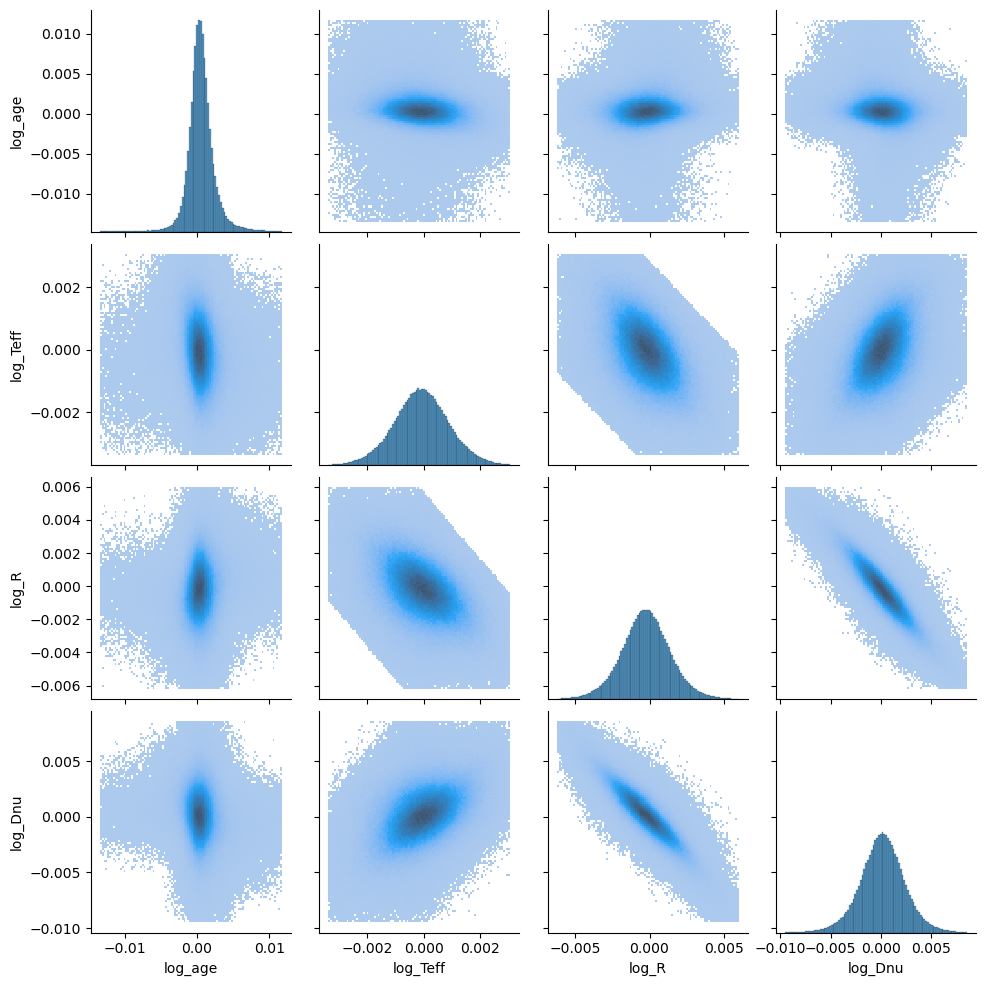
\includegraphics[width=1.0\linewidth]{figures/error.png}
    \caption{The error \(\vec\error_i = \vec\outputs_i - \vec\pred_i\) of the emulator predictions evaluated on the test dataset. TODO: replace with plot without data cut.}
    \label{fig:error}
\end{figure}

\subsection{Hierarchical Bayesian model}
\label{sec:hbm}

%
\begin{equation}
    p(\vec \theta_i, \vec \phi \mid \vec\obs_i) \propto p(\vec\obs_i \mid \vec \theta_i) \, p(\vec\theta_i \mid \vec\phi) \, p(\vec\phi),
\end{equation}
%

\subsubsection{Likelihood}

We approximate the emulator error (\(\vec\delta\)) across the test dataset with a multivariate student's t-distribution, \(\tdist(\delta \mid \nu_\delta, \vec\mu_\delta, \mat\Sigma_\delta)\). This can be decomposed into a multivariate normal distribution with its covariance scaled by a gamma-distributed scale parameter \(\sigma^{-2}\).
%
\begin{equation}
    p(\vec\error_i \mid \nu_\delta, \vec\mu_\delta, \mat\Sigma_\delta) = \gammadist(\sigma_i^{-2} \mid \frac{\nu_\delta}{2}, \frac{\nu_\delta}{2}) \, \normaldist(\vec\error_i \mid \vec\mu_\delta, \sigma_i^2 \mat\Sigma_\delta),
\end{equation}
%
We propagate this error to our model likelihood,
%
\begin{equation}
    p(\vec\obs_i \mid \vec\theta_i) = \normaldist(\vec\obs_i \mid \vec\mu_i, \mat\Sigma_i)
\end{equation}
%
where the observable quantities are a linear transformation of the emulator outputs,
%
\begin{align}
    \vec\mu_i &= \mat A \, (\vec\pred_i + \vec\mu_\delta) + \vec b\\
    \mat\Sigma_i &= \sigma_i^2 \, \mat{A} \, \mat{\Sigma}_\delta \, \mat{A}^{\transpose} + \sigma_{y,i}^2 \, \mat{I} \label{eq:covariance}
\end{align}
%
and \(\mat A\) is a matrix converting the emulator output to observed quantities.

In this work, we consider observing \(\teff[i]\), \(L_i\), and \(\Delta\nu\) with uncertainties of 2 per cent, 2 per cent, and 1 per cent respectively. In other words, we assume the likelihood to be normally distributed centred on the observed values and scaled by their uncertainties. However, the emulator outputs logarithmic quantities, making the transformation from \(\pred_i\) to observables non-linear. Since the observation noise is small, the logarithm of the observed quantities is also approximately normally distributed. Therefore, we transform the observables and their standard deviations to logarithmic space and continue. In other words, we observe \(\vec\obs_i = [\log\teff[i], \log L_i, \log\Delta\nu_i]\) with uncertainty \(\vec\sigma_{y, i} \approx [0.02, 0.02, 0.01] / \ln(10)\).

\begin{equation}
    \mat A = 
    \begin{bmatrix}
        0 & 1 & 0 & 0\\
        0 & 4 & 2 & 0\\
        0 & 0 & 0 & 1
    \end{bmatrix}
    , \quad
    \vec b =
    \begin{bmatrix}
        0\\
        - 4 \log \teff[\odot]\\
        0
    \end{bmatrix}
\end{equation}


\subsubsection{Prior}

\begin{equation}
    \begin{split}
        p(\vec{\theta} \mid \vec\phi) = \sum_i \, &\normaldist(Y_i \mid \mu_Y, \sigma_Y^2) \, \normaldist(\mlt[i] \mid \mu_\alpha, \sigma_\alpha^2) \\
        &\times p(\eep_i, M_i, \feh_i)
    \end{split}
\end{equation}
%
where,
%
\begin{align}
    \mu_Y &= \frac{\yp + f}{1 + f}, \\
    f &= \frac{\dydz}{Z / X + 1}, \\
    \log({Z}/{X}) &= \feh + \log({Z}/{X})_\odot,
\end{align}
%
where \((Z/X)_\odot = 0.0181\).

%
\begin{equation}
    \begin{split}
        p(\vec\phi) &= \normaldist(\yp \mid 0.247, 0.001) \, \uniformdist(\dydz \mid 0.0, 3.0) \\
        &\times \gammadist(\sigma_Y^{-2} \mid 3, 10^{-4}) \, \uniformdist(\mu_\alpha \mid 1.5, 2.5) \\
        &\times \gammadist(\sigma_\alpha^{-2} \mid 3, 10^{-2})
    \end{split}
\end{equation}

\begin{figure}
    \centering
    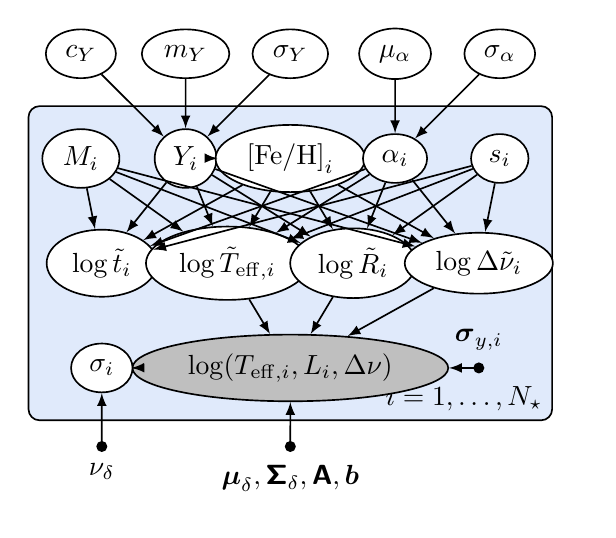
\begin{tikzpicture}[scale=1.33, line width=0.6pt, every node/.style={ellipse, draw, fill=white}, >=latex]
    % Hyperparameters
    \node (ay) at (0, 5) {$\yp$};
    \node (by) at (1, 5) {$\dydz$};
    \node (sy) at (2, 5) {$\sigma_Y$};
    \node (ma) at (3, 5) {$\mu_\alpha$};
    \node (sa) at (4, 5) {$\sigma_\alpha$};

    % Plate - Individual star
    \draw[fill=CornflowerBlue!20, rounded corners] (-0.5, 1.5) rectangle (4.5, 4.5);
    % \draw[fill=JungleGreen!20, rounded corners] (-0.5, 1.5) rectangle (4.5, 4.5);
    % \node[draw=none, fill=none, rotate=90, above, align=left, anchor=south west] at (-0.5, 1.5) {Individual\\Star};
    \node[draw=none, fill=none, above left, align=right] at (4.5, 1.5) {$i = 1, \dots, N_\star$};

    % Input parameters
    \node (mi) at (0, 4) {$M_i$};
    \node (yi) at (1, 4) {$Y_i$} edge [<-] (ay) edge [<-] (by) edge [<-] (sy);
    \node (fehi) at (2, 4) {$\feh_i$} edge [->] (yi);
    \node (ai) at (3, 4) {$\alpha_i$} edge [<-] (ma) edge [<-] (sa);
    \node (eepi) at (4, 4) {$\eep_i$};

    % Output parameters
    % \node (age) at (0, 3) {$t_i$};
    % \node [fill=black!25] (teff) at (1, 3) {$T_{\mathrm{eff}, i}$};
    % \node [fill=black!25] (lum) at (2, 3) {$L_i$} edge [<-] (teff);
    % \node (rad) at (3, 3) {$R_i$} edge [->] (lum);
    % \node (dnu) at (4, 3) {$\Delta\nu_i$};
    \node (age) at (0.2, 3) {$\log \tilde t_i$};
    \node (teff) at (1.4, 3) {$\log \tilde T_{\mathrm{eff}, i}$};
    \node (rad) at (2.6, 3) {$\log \tilde R_i$};
    \node (dnu) at (3.8, 3) {$\log \Delta\tilde\nu_i$};

    % Connect neural network inputs and outputs
    \foreach \x in {mi, yi, fehi, ai, eepi}
    \foreach \y in {age, teff, rad, dnu}
    \draw[->] (\x) -- (\y);

    \node [fill=black!25] (obs) at (2, 2) {$\log(\teff[i], L_i, \Delta\nu)$} edge [<-] (teff) edge [<-] (rad) edge [<-] (dnu);
    % Plate - Emulator noise
    % \draw[fill=BurntOrange!20, rounded corners] (-0.5, 0.4) rectangle (1.5, 1.4);
    % \node[draw=none, fill=none, rotate=90, above, align=left, anchor=south west] at (-0.5, 0.4) {Emulator\\Error};
    % \node[draw=none, fill=none, above left, align=right] at (1.5, 0.4) {$j = 1, \dots, N_\mathrm{out}$};

    % Emulator uncertainty
    % \node (sig) at (1, 0.9) {$\sigma_j$} edge [->] (teff) edge [->] (lum);
    % \fill (0, 0.9) circle (1.5pt) edge [->] (sig) node[above, fill=none, draw=none] (slum) {$\tau_j$};
    % \fill (2, 0.9) circle (1.5pt) edge [->] (sig) node[above, fill=none, draw=none] (slum) {$\nu$};

    % \node (sig) at (1, 1) {$u$} edge [->] (teff) edge [->] (lum);
    % \fill (0, 1) circle (1.5pt) edge [->] (sig) node[above, fill=none, draw=none] (slum) {$\nu, \vec{\tau}$};

    % \node (sig) at (1, 2) {$\Sigma_i$} edge [->] (teff) edge [->] (lum);

    % \node (sig) at (1, 2) {$\mat\Sigma_i$} edge [->] (obs);

    \node (sig) at (0.2, 2) {$\sigma_i$} edge [->] (obs);

    % \fill (1, 1) circle (1.5pt) edge [->] (sig) node[right, fill=none, draw=none] (slum) {$\nu, \vec{\tau}$};

    % Observational Uncertainty
    % \fill (0, 2) circle (1.5pt) edge [->] (sig) node[below, fill=none,draw=none] {$\sigma_{T_\mathrm{eff}, i}$};
    % \fill (2, 2) circle (1.5pt) edge [->] (sig) node[below, fill=none, draw=none] {$\sigma_{L, i}$};
    
    % \fill (0, 2) circle (1.5pt) edge [->] (sig) node[below, fill=none,draw=none] {$\sigma_{z, i}$};
    % \fill (1, 1) circle (1.5pt) edge [->] (sig) node[below, fill=none,draw=none] {$\nu_\delta, \mat\Sigma_\delta$};
    % \fill (2, 1) circle (1.5pt) edge [->] (obs) node[below, fill=none,draw=none] {$\vec\mu_\delta$};
    
    \fill (3.8, 2) circle (1.5pt) edge [->] (obs) node[above, fill=none,draw=none] {$\vec\sigma_{y, i}$};
    \fill (2, 1.25) circle (1.5pt) edge [->] (obs) node[below, fill=none,draw=none] {$\vec\mu_\delta, \mat\Sigma_\delta, \mat A, \vec b$};
    \fill (0.2, 1.25) circle (1.5pt) edge [->] (sig) node[below, fill=none,draw=none] {$\nu_\delta$};

    % \draw [decorate,decoration={brace,amplitude=4pt}]
    % (4.66, 5.25) -- (4.66, 4.75) node[fill=none,draw=none,midway,right]{$\vec\phi$};
    % \draw [decorate,decoration={brace,amplitude=4pt}]
    % (4.66, 4.25) -- (4.66, 3.75) node[fill=none,draw=none,midway,right]{$\inputs_i$};
    % \draw [decorate,decoration={brace,amplitude=4pt}]
    % (4.66, 3.25) -- (4.66, 2.75) node[fill=none,draw=none,midway,right]{$\pred_i$};

\end{tikzpicture}

    \caption{A probabilistic directed acyclic graph showing the relationship between parameters in the model. Arrows show the direction of dependence.
    % Parameters surrounded by a solid and dotted lines are probabilistic and deterministic respectively.
    Parameters shaded grey are observed and those represented by black dots are fixed. 
    % Dashed lines group parameters which are inputs to or outputs from other routines (e.g. the neural network).
    The blue box groups parameters which loop over \(i\). Definitions of the parameters and their description are given in the text.
    }
\end{figure}

\begin{figure}
    \centering
    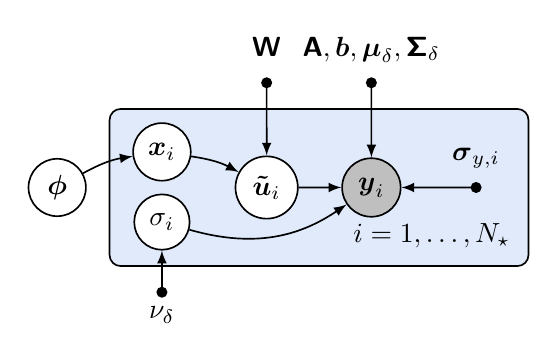
\begin{tikzpicture}[scale=1.33, line width=0.6pt, every node/.style={circle, draw, fill=white}, >=latex]

    \draw[fill=CornflowerBlue!20, rounded corners] (0.5, 0.25) rectangle (4.5, 1.75);
    \node[rectangle, draw=none, fill=none, above left=3pt, align=right] at (4.5, 0.25) {$i = 1, \dots, N_\star$};
    \node (hyper) at (0, 1) {$\vec\phi$};
    \node (inputs) at (1, 1.34) {$\vec\inputs_i$} edge [<-, bend right=10] (hyper);
    \node (error) at (1, 0.67) {$\sigma_i$};
    \node (outputs) at (2, 1) {$\vec\pred_i$} edge [<-, bend right=10] (inputs);
    \node [fill=black!25] (observables) at (3, 1) {$\vec\obs_i$} edge [<-] (outputs) edge [<-,bend left=25] (error);

    \fill (1, 0) circle (1.5pt) edge [->] (error) node[below=3pt, fill=none,draw=none, rectangle, text height=3pt] {$\nu_\error$};
    \fill (2, 2) circle (1.5pt) edge [->] (outputs) node[above=3pt, fill=none,draw=none, rectangle, text depth=3pt] {$\mat W$};
    \fill (3, 2) circle (1.5pt) edge [->] (observables) node[above=3pt, fill=none,draw=none, rectangle, text depth=3pt] {$\mat A, \vec b, \vec\mu_\error, \mat\Sigma_\error$};
    \fill (4, 1) circle (1.5pt) edge [->] (observables) node[above=3pt, fill=none,draw=none, rectangle, text depth=3pt] {$\vec\sigma_{\obs, i}$};

\end{tikzpicture}


    \caption{A probabilistic directed acyclic graph showing the relationship between parameters in the model. Arrows show the direction of dependence.
    % Parameters surrounded by a solid and dotted lines are probabilistic and deterministic respectively.
    Parameters shaded grey are observed and those represented by black dots are fixed. 
    % Dashed lines group parameters which are inputs to or outputs from other routines (e.g. the neural network).
    The blue box groups parameters which loop over \(i\). Definitions of the parameters and their description are given in the text.
    }
\end{figure}

\subsection{Synthetic stars}
\label{sec:synth}

\begin{itemize}
    \item Truths from above model
    \item Synthetic stars pulled from Yagaung Li's grid
\end{itemize}


\section{Results}
\label{sec:results}

\section{Discussion}
\label{sec:discussion}

\section{Conclusion}
\label{sec:conclusion}

\section*{Acknowledgements}

The Acknowledgements section is not numbered. Here you can thank helpful
colleagues, acknowledge funding agencies, telescopes and facilities used etc.
Try to keep it short.

%%%%%%%%%%%%%%%%%%%%%%%%%%%%%%%%%%%%%%%%%%%%%%%%%%
\section*{Data Availability}
 
The inclusion of a Data Availability Statement is a requirement for articles published in MNRAS. Data Availability Statements provide a standardised format for readers to understand the availability of data underlying the research results described in the article. The statement may refer to original data generated in the course of the study or to third-party data analysed in the article. The statement should describe and provide means of access, where possible, by linking to the data or providing the required accession numbers for the relevant databases or DOIs.

%%%%%%%%%%%%%%%%%%%% REFERENCES %%%%%%%%%%%%%%%%%%

% The best way to enter references is to use BibTeX:

\bibliographystyle{mnras}
\bibliography{references} % if your bibtex file is called example.bib

% Alternatively you could enter them by hand, like this:
% This method is tedious and prone to error if you have lots of references
%\begin{thebibliography}{99}
%\bibitem[\protect\citeauthoryear{Author}{2012}]{Author2012}
%Author A.~N., 2013, Journal of Improbable Astronomy, 1, 1
%\bibitem[\protect\citeauthoryear{Others}{2013}]{Others2013}
%Others S., 2012, Journal of Interesting Stuff, 17, 198
%\end{thebibliography}

%%%%%%%%%%%%%%%%%%%%%%%%%%%%%%%%%%%%%%%%%%%%%%%%%%

%%%%%%%%%%%%%%%%% APPENDICES %%%%%%%%%%%%%%%%%%%%%

\appendix

%%%%%%%%%%%%%%%%%%%%%%%%%%%%%%%%%%%%%%%%%%%%%%%%%%

% Don't change these lines
\bsp	% typesetting comment
\label{lastpage}
\end{document}

% End of mnras_template.tex
